\documentclass[runningheads]{llncs}

\usepackage[utf8]{inputenc}
\usepackage[T1]{fontenc}
\usepackage{graphicx}
\graphicspath{{Figures/}}
\usepackage{tikz}
\usetikzlibrary{shapes.geometric, arrows.meta, positioning, fit, calc, backgrounds}
\usepackage[round]{natbib}
\usepackage{verbatim}
\usepackage{multirow}
\usepackage{amsmath, amssymb}
\usepackage{booktabs}
\usepackage{hyperref}
\hypersetup{urlcolor=blue, colorlinks=true}

% Standard LNCS packages and setup
\title{Spatiotemporal Deepfake Detection via Texture-Enhanced Multi-Attentional ResNeXt50-LSTM Architecture}
\titlerunning{Spatiotemporal Deepfake Detection}

\author{Aarav Rajput\inst{1} \and Trapti Sharma\inst{1} \and Rajit Nair\inst{1} \and Hasan Alkahtani\inst{2} \and Adel Musaad Alrasheedi\inst{3} \and  Sami Morsi\inst{4} \and Ahmed A.F.\ Osman\inst{4} \and *Theyazn H.H.\ Aldhyani\inst{4}}
\authorrunning{A. Rajput et al.}

\institute{School of Computer Science Engineering and Artificial Intelligence\\ VIT Bhopal University, Kothrikalan, Sehore, Madhya Pradesh, 466114, India\\
\email{aarav.rajput2021@vitbhopal.ac.in}, \email{trapti16sharma@gmail.com}, \email{rajitnitbpl@gmail.com}
\and
College of Computer Science and Information Technology, King Faisal University, P.O.\ Box 400, Al-Ahsa, 31982, Saudi Arabia.\\
\email{hsalkahtani@kfu.edu.sa}
\and
Ministry of Education, Riyadh \\
\email{adelmr8989@gmail.com}
\and
Applied College, King Faisal University, Al-Ahsa, 31982, Saudi Arabia\\
\email{smorsi@kfu.edu.sa}, \email{afadol@kfu.edu.sa}, \email{*taldhyani@kfu.edu.sa}
}

\begin{document}

\maketitle

\begin{abstract}
\textbf{Purpose:} This paper addresses the challenge of deepfake video and image detection across diverse generator types. Current detectors often struggle to generalize because they over-specialize on outdated datasets or specific artifacts (such as blending boundaries) that are absent in modern Entire Face Synthesis (EFS).

\textbf{Design/methodology/approach:} We propose a spatiotemporal deepfake detection framework that leverages a ResNeXt50 convolutional neural network for spatial feature extraction, integrated with a Long Short-Term Memory (LSTM) network to model temporal sequence dependencies. The framework incorporates a shallow Texture Enhancement Block (TEB) to capture high-frequency textural traces and a multi-attentional mechanism with Bilinear Attention Pooling (BAP) to extract regional descriptors from independent facial zones. We train the network using a composite loss function that pairs cross-entropy with a Regional Independence Loss ($\mathcal{L}_{RIL}$) to prevent attention collapse.

\textbf{Findings:} Evaluated using 5-fold cross-validation on the DF40 and FaceForensics++ benchmarks, the proposed framework demonstrates superior detection accuracy and generalization capabilities. In cross-domain evaluations on unseen generator categories, it outperforms state-of-the-art baseline detectors (including CLIP-large and UniFace) by a significant margin (e.g., achieving $83.2\% \pm 0.4\%$ AUC on EFS when trained on Face Reenactment, outperforming CLIP-large by $+2.3\%$). Paired t-tests with Bonferroni and Benjamini-Hochberg FDR corrections confirm that these improvements are statistically significant ($p < 0.05$).

\textbf{Originality/value:} Unlike existing spatial-only or globally-pooled detectors, our approach introduces a unified spatiotemporal architecture that preserves shallow frequency cues and enforces regional independence across attention heads, preventing them from collapsing onto a single dominant facial region.

\textbf{Implications:} Our work shows that combining regional attention diversity with sequential temporal modeling is crucial for robust forensic analysis. It highlights the necessity of demographic subgroup calibration and the auditing of detector robustness against compression and modern diffusion generators to ensure fair and secure real-world deployment.

\keywords{Deepfake Detection \and Spatiotemporal \and CNN-LSTM \and Multi-Attentional \and Texture Enhancement}
\end{abstract}

\section{Introduction}
\label{sec:introduction}

\subsection{Background and Motivation}
A decade ago, generating high-fidelity facial swaps in video sequences required specialized visual effects teams and substantial computational rendering clusters. Today, commodity graphics hardware and publicly accessible pre-trained models enable users to synthesize realistic manipulations with minimal resource constraints. This democratization of generative tools has elevated deepfake detection to a critical research area rather than a mere digital curiosity. While the underlying spatiotemporal techniques support legitimate industries such as multilingual film synchronization and video game animation, they also present significant risks when deployed to generate unauthorized and deceptive content featuring real individuals.

The first deepfakes appeared in late 2017. They used autoencoders to swap faces and circulated on anonymous forums. Within about a year, GANs replaced autoencoders and the quality jumped sharply. Diffusion models came next and currently produce the most convincing results \citep{Liu2025Evolving, Shiohara2025ExposeAnyone}. Each step also widened what could be faked. The current tools do four distinct things. They swap one face for another, drive a target face with the expressions and head movements of a source, synthesize a face that belongs to no real person, and edit attributes like apparent age or gender on an existing face. By 2026, the output of these tools was good enough that a viewer cannot reliably tell it apart from genuine footage by eye \citep{Liu2025SIDA}.

This is already causing real harm. Fabricated video has been used to put words in the mouths of politicians. Fraudsters have cloned a person's face and voice to defeat the video checks banks use to verify identity. People have been targeted with fake explicit imagery built from ordinary photos of them. A convincing fake travels further and faster than the correction that follows it, which is why digital media forensics treats reliable detection as urgent rather than academic.

The first detectors were CNNs that classified single frames as real or fake. Against the generators of that period they worked, because those generators left visible traces: seams where a swapped face was blended in, mismatched resolution between the face and the rest of the frame, smeared texture around the hairline. Then the generators got better and stopped leaving those traces. A detector trained to spot blending seams has nothing to spot once the seams are gone.

\subsection{Problem Statement}
Detection has not kept up with generation, and it has fallen behind in three particular ways. Each one is the reason for a design decision later in this paper.

\subsubsection{The Generalization Gap}
A detector trained on one kind of forgery tends to fail on the others. FaceForensics++ (FF++) is still the most common training benchmark, even though the forgery methods it contains are several years out of date \citep{roessler2019faceforensicspp, Yan2023DeepfakeBench}. A model that has learned to find blending boundaries has nothing to work with on Entire Face Synthesis (EFS) from a diffusion model, because that kind of forgery has no blending boundary \citep{Yan2024DF40}. The comparison problem makes this harder to see. Papers report results under different preprocessing and training setups, so two numbers in two papers are often not measuring the same thing. Run the same model under different setups and the AUC can move by several points. Yan et al. went through this carefully, and the size of the gap they found was larger than most researchers in the area had assumed \citep{Deng2025DeepfakeEval}.

\subsubsection{Temporal Inconsistencies}
Although deepfakes are inherently temporal video sequences, many existing detectors analyze frames independently, discarding temporal context. Analyzing isolated frames using spatial-only models often fails to detect manipulation, as advanced generative models excel at producing realistic individual frames. However, these models frequently introduce inter-frame inconsistencies, such as unnatural blinking rhythms, subtle movement jitter at transition boundaries, and premature expression transitions. Because these dynamic discrepancies are invisible in static frames, robust detection necessitates sequence-level modeling.

\subsubsection{Fine-Grained Artifacts}
A good forgery does not look wrong everywhere at once. It looks wrong in one place. The corner of an eye, the line where skin meets hair, the texture of a small patch of cheek. A detector that squeezes the whole face into one feature vector and runs a yes/no classifier on it will smear that one bad spot together with everything that looks fine, and the signal gets lost in the average. Framing the task as fine-grained classification, where the model attends to specific regions instead of the whole image at once, is a better fit for the kind of mistake current generators actually make \citep{Zhao2021MultiAttentional, Chen2024FreqNet}.

\subsection{Proposed Approach and Methodological Innovations}
The framework proposed in this paper addresses these three limitations through a unified spatiotemporal architecture built on three synergistic methodological innovations:

\begin{enumerate}
    \item \textbf{Spatiotemporal Texture-Attentional Integration:} Unlike prior works that use temporal sequence modeling or multi-attention in isolation, our approach formulates a dynamic sequence representation. Shallow-layer Texture Enhancement (TEB) features are fused with regional Bilinear Attention Pooling (BAP) descriptors before sequence aggregation through an LSTM network. This preserves high-frequency microscopic artifacts through deep pooling layers and models inter-frame temporal inconsistencies simultaneously.
    
    \item \textbf{Fourier-Domain Frequency Preservation \& Diversity Augmentation:} To protect high-frequency texture traces from degradation by standard video compression or spatial augmentations, we implement a Fourier-space frequency-preserving augmentation strategy paired with Regional Independence Loss ($\mathcal{L}_{RIL}$). This prevents attention heads from collapsing into a single global descriptor and retains discriminative frequency cues across diverse forgery types.
    
    \item \textbf{Standardized Cross-Generator Evaluation Protocol:} We conduct rigorous within-domain and cross-generator evaluation across 40 distinct manipulation algorithms using the DF40 dataset, establishing standardized benchmark protocols against state-of-the-art detectors under identical pre-training and augmentation conditions.
\end{enumerate}

\subsection{Contributions}
Specifically, this paper makes three key contributions:

\begin{itemize}
    \item \textbf{Architectural Innovation:} We present a novel unified detection framework combining ResNeXt50 spatial feature extraction, shallow texture enhancement, multi-attentional regional pooling, and LSTM sequence modeling. We demonstrate through rigorous k-fold cross-validation with statistical significance ($\text{Mean} \pm \text{Std Dev}$) that this end-to-end integration outperforms both spatial-only and unconstrained temporal baselines.
    \item \textbf{Fine-Grained Multi-Region Feature Disambiguation:} We reframe deepfake detection as a multi-region fine-grained classification task. By enforcing a Regional Independence Loss and Attention Guided Data Augmentation (AGDA), we prevent attention collapse and ensure distinct coverage across local facial parts (eyes, nose, mouth, boundary).
    \item \textbf{Comprehensive DF40 Benchmark \& SOTA Comparisons:} We provide an exhaustive empirical evaluation on the 40-method DF40 dataset across Face Swapping, Face Reenactment, Entire Face Synthesis, and Face Editing, benchmarking against state-of-the-art detectors (CLIP-large, UniFace, SBI, Xception) under strictly controlled training pipelines.
\end{itemize}

\subsection{Paper Structure}
The remainder of this paper is organized as follows: Section \ref{sec:lit_review} reviews the deepfake generation and detection literature. Section \ref{sec:methodology} describes the proposed ResNeXt50-LSTM multi-attentional architecture, mathematical formulations, and training strategy in detail. Section \ref{sec:results} presents the experimental setup, benchmark results on DF40 and FF++, ablation studies, hyperparameter sensitivity analysis, quantitative failure case breakdowns, and ethical considerations. Section \ref{sec:conclusion} concludes the paper and outlines future research directions.

\section{Literature Review}
\label{sec:lit_review}

\subsection{Overview}
Research interest in deepfake detection accelerated sharply from 2018 onward, driven by high-profile misuse cases. \citet{Rana2022Systematic} mapped the field systematically in their comprehensive survey, identifying four detection categories: deep learning-based, conventional machine learning, statistical, and blockchain-based approaches. Deep learning methods account for roughly 77\% of published work, which makes sense given that the generation methods being targeted are themselves neural \citep{Wang2025MultimodalSurvey}.

This section traces the generation technology that detectors must contend with, then examines four bodies of work that motivated this paper: DeepfakeBench's benchmarking critique, DF40's generalization analysis, Zhao et al.'s fine-grained spatial approach, and Jugade et al.'s temporal modeling study. The recurring theme across all four is that detection performance reported in isolation tells you very little about how a detector will behave in practice.

\subsection{The Evolution of Deepfake Generation}
Detection and generation have evolved in close response to each other. Understanding what each generation of synthesis tools produces, and what it fails to conceal, is prerequisite to understanding why current detectors work when they do.

\subsubsection{Autoencoder-Based Face Swapping}
Early deepfakes, including FakeApp and DeepFaceLab, used shared autoencoder architectures. Two encoders with shared weights learn a common latent representation of two faces; separate decoders reconstruct each identity from that shared space. The results were technically novel for their time but visually imperfect. Hair boundaries blurred. Skin-tone transitions were inconsistent. High-frequency texture detail was lost. These were exploitable artifacts, and early detectors were built to find exactly them.

\subsubsection{Generative Adversarial Networks (GANs)}
StyleGAN and its successors changed the situation. A min-max game between generator and discriminator drove both toward higher quality, and state-of-the-art GAN swappers like SimSwap and InSwapper achieved identity transfers that held up to closer inspection. They were not perfect. GAN upsampling layers introduce characteristic ``checkerboard'' patterns in the frequency domain, a byproduct of how transposed convolutions operate. Frequency-based detectors learned to find these, turning a generation artifact into a detection handle \citep{Zhao2021MultiAttentional, Sun2024ForgeryTrace}.

\subsubsection{Diffusion Models (DDPM and LDM)}
Denoising Diffusion Probabilistic Models and Latent Diffusion Models raised the quality ceiling again by reversing a Gaussian noise process rather than training a discriminator. The images produced show greater diversity and fewer structural artifacts than GAN outputs. The checkerboard problem does not appear. What does appear is a different kind of high-frequency noise signature, distinct from GAN traces, that requires detection systems to generalize across two fundamentally different artifact distributions \citep{Yan2024DF40, Li2024DiffSeg, Shiohara2025ExposeAnyone}.

\subsection{Benchmarking and Standardization Challenges}
One of the field's more uncomfortable findings is that a significant portion of reported performance gains may not reflect genuine methodological advances. \citet{Yan2023DeepfakeBench} documented this through the DeepfakeBench study. Differences in preprocessing choices, data augmentation pipelines, and pre-training protocols produce performance differences large enough to dwarf the claimed improvements of proposed methods. Two papers evaluating the same detector on the same dataset can report results several AUC points apart simply because their training pipelines differ.

\subsubsection{The Role of Naive Detectors}
The counterintuitive finding from DeepfakeBench is that standard CNNs — Xception being the representative case — perform comparably to architectures marketed as state-of-the-art when training conditions are held constant. Xception reached an AUC of 94.50\% in within-domain evaluation, roughly matching specialized frequency-based detectors \citep{Chen2024FreqNet}. The implication is uncomfortable but important: many published performance gaps likely reflect differences in augmentation schemes and pre-training choices, not the architectural innovations being claimed. The proposed method looks better than the baseline partly because it was trained more carefully.

\subsubsection{The Effect of Data Augmentation}
The DeepfakeBench study \citep{Yan2023DeepfakeBench} provides specific evidence of this through its augmentation analysis. Compression and Gaussian blur augmentation improve resilience to low-quality video, but they degrade frequency-based detectors by masking the high-frequency signal those methods depend on. This is a real design constraint, not an edge case. An augmentation strategy that protects against one failure mode can directly create another. The balanced approach, preserving frequency information while building resilience to spatial degradation, requires explicit attention \citep{Huang2024FreqBlender}.

\subsection{The Generalization Gap and Dataset Diversity}
Cross-generator generalization is where the practical failure of current detectors is most visible. The DF40 benchmark \citep{Yan2024DF40} tested what happens when detectors trained on standard datasets encounter generation methods not represented in their training data. The results were poor across the board.

\begin{table}[ht]
    \centering
    \caption{Comparative Analysis of Major Deepfake Datasets}
    \label{tab:dataset_comparison}
    \resizebox{\textwidth}{!}{
    \begin{tabular}{l|c|c|l}
        \toprule
        \textbf{Dataset} & \textbf{Year} & \textbf{Videos/Images} & \textbf{Key Features} \\
        \midrule
        FaceForensics++ \citep{roessler2019faceforensicspp} & 2019 & 5,000 videos & Standardized for FS and FR. \\
        Celeb-DF (v2) \citep{Celeb_DF_cvpr20} & 2020 & 6,229 videos & High-quality swaps with minimized artifacts. \\
        DFDC \citep{Dolhansky2020DFDC} & 2020 & 128,454 videos & Large scale, real-world perturbations. \\
        WildDeepfake \citep{Zi2020WildDeepfake} & 2021 & 7,314 videos & Collected from internet sources. \\
        \textbf{DF40} \citep{Yan2024DF40} & \textbf{2024} & \textbf{40 methods} & \textbf{Unparalleled diversity of generation techniques.} \\
        \bottomrule
    \end{tabular}
    }
\end{table}

\subsubsection{Asymmetric Failure Modes}
DF40 covers 40 distinct manipulation methods across Face Swapping (FS), Face Reenactment (FR), Entire Face Synthesis (EFS), and Face Editing (FE). The diversity revealed a pattern that straight accuracy numbers obscure: performance degrades unevenly across categories. Models trained on Face Swapping generalize reasonably well to Entire Face Synthesis. Models trained on EFS have significant trouble with localized Face Swapping. The mechanism is that EFS-trained models learn to identify global artifacts, while FS artifacts are localized to the face boundary. Train on one, the other category's signal is invisible.

\subsubsection{Non-Blending Artifacts}
A consequence of how modern generators work is that the detection heuristics embedded in older methods simply do not apply. Systems like SimSwap and diffusion-based methods synthesize the complete image without traditional compositing steps. There is no blending boundary to find. Detectors that use blending seams as their primary signal will classify these outputs as real by default. DF40 also showed that large pre-trained models like CLIP transfer better to unseen generator types than standard backbones, likely because pre-training on large-scale real-world data builds richer representations of human facial structure.

\subsection{Fine-Grained Spatial Analysis}
\citet{Zhao2021MultiAttentional} argued that treating deepfake detection as a binary classification problem is the wrong framing. The discriminative signal in high-quality forgeries is local, not global. Global feature extraction pools over the entire face image; it will average out a subtle artifact at the left eye corner the same way it averages out the background wall. Reframing detection as a fine-grained classification problem, where the model must identify \textit{which parts} of the face are anomalous, is structurally better suited to the task.

\subsubsection{Multi-Attentional Framework}
Zhao et al.'s implementation uses multiple parallel spatial attention heads, each directed toward a different facial region. The eyes, lips, and face boundaries can carry different forgery signals simultaneously; separate attention heads allow the network to attend to each without forcing a single global descriptor to encode everything. The key design insight is that forgery evidence is distributed, and a detector should distribute its attention accordingly.

\subsubsection{Texture Enhancement and Regional Independence}
Manipulation traces tend to be high-frequency signals that get suppressed as features pass through deeper layers and pooling operations. \citet{Zhao2021MultiAttentional} added a texture enhancement block operating on shallow feature maps, before pooling has a chance to destroy the relevant detail — a choice that subsequent work on wavelet sub-band analysis supports \citep{Zhu2025WaveDIF, Li2024FrequencyAware}. A Regional Independence Loss prevents attention heads from collapsing onto the same location. Without it, multiple heads will converge on whichever facial region carries the strongest signal, effectively reducing the multi-head system to a single-head one \citep{pan25}. The loss, combined with Attention Guided Data Augmentation (AGDA), keeps heads discriminatively separate.

\subsection{Video Forensics: Modeling Time}
A spatial detector is, by construction, a frame-level detector. \citet{Jugade2026SpatialTemporal} showed the gap this creates: spatial-only systems miss inter-frame jitter, anomalous blink sequences, and other temporal inconsistencies that only appear across a sequence of frames. Work on facial component-guided adaptation in foundation models corroborates this, showing that attending to specific facial regions over time improves generalization in video-based detection \citep{Zhang2025FCG}.

\subsubsection{CNN-LSTM Hybrid Architectures}
The hybrid approach Jugade et al. evaluated is conceptually straightforward: a CNN extracts spatial features from each frame, and an LSTM models how those features change over time. The integration is where design choices matter. The CNN selection affects what spatial information is available to the LSTM. Different backbones produce meaningfully different results.

\subsubsection{Performance Trade-offs}
The comparative results from Jugade et al. are practically useful for backbone selection. VGG16-LSTM achieved high training accuracy (99.16\%) and recall (94.40\%), but showed clear overfitting — training and validation accuracy diverge noticeably. ResNeXt50-LSTM reached 94.23\% precision with better generalization. For a detection task where deployment performance matters more than in-sample fit, ResNeXt50's stability across training and validation is the more relevant quality.

\subsection{Motivations for the Proposed Model}
The four bodies of work reviewed here each point to a specific design decision in this paper:

\begin{enumerate}
    \item \textbf{Fine-grained detection (from Zhao et al.):} The proposed model frames detection as a fine-grained problem, not binary classification. Multi-attentional mechanisms with texture enhancement blocks preserve localized, high-frequency cues at the eyes and lips that global pooling would erase.

    \item \textbf{Hybrid spatiotemporal modeling (from Jugade et al.):} An LSTM is added above the spatial backbone to capture inter-frame anomalies. ResNeXt50 is selected based on its demonstrated stability in the hybrid architecture comparison.

    \item \textbf{Standardized training protocols (from Yan et al. — DeepfakeBench):} Training procedures are held consistent across all experiments. Augmentation (compression, blur) is chosen to build resilience to real-world degradation without destroying the frequency artifacts the texture module depends on.

    \item \textbf{Diversity-aware training (from Yan et al. — DF40):} Training covers Face Swapping, Reenactment, and Entire Face Synthesis explicitly. Non-blending deepfakes such as SimSwap outputs are included to prevent the model from over-specializing on boundary artifacts that newer generators simply do not produce.
\end{enumerate}

\section{Methodology}
\label{sec:methodology}

\subsection{Overview of the Proposed Spatiotemporal Framework}
The design of this architecture addresses the primary vulnerabilities of existing deepfake detectors: susceptibility to unseen generator artifacts due to global feature pooling and insensitivity to inter-frame temporal incoherence. The framework operates across three coordinated phases: Preprocessing and Data Standardization (Phase 1), Spatial Feature Extraction with Texture Enhancement and Multi-Attentional Bilinear Pooling (Phase 2), and Temporal Sequence Modeling with Classification (Phase 3). The spatial stage leverages a ResNeXt50 convolutional neural network augmented with a shallow Texture Enhancement Block (TEB) and multi-head attention inspired by fine-grained visual classification \citep{Zhao2021MultiAttentional}. The temporal stage utilizes a multi-layer Long Short-Term Memory (LSTM) network to capture dynamic transition anomalies across sequential frames \citep{Jugade2026SpatialTemporal}.

\begin{figure}[ht]
    \centering
    \resizebox{\textwidth}{!}{

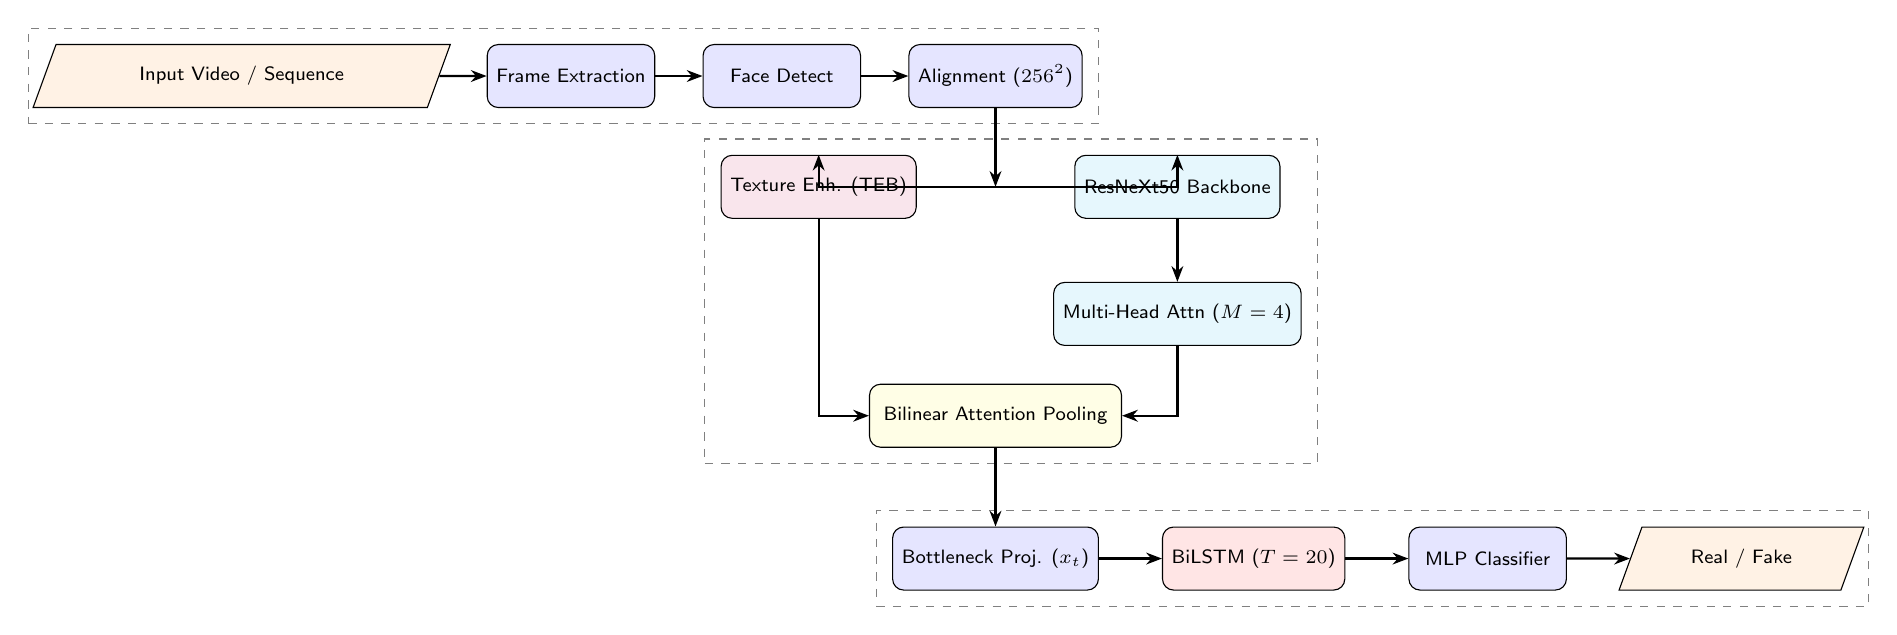
\begin{tikzpicture}[
    node distance=1.2cm and 1.2cm,
    font=\sffamily\scriptsize,
    process/.style={
        rectangle,
        minimum width=2.0cm,
        minimum height=0.8cm,
        text centered,
        draw=black,
        fill=blue!10,
        rounded corners
    },
    io/.style={
        trapezium,
        trapezium left angle=70,
        trapezium right angle=110,
        minimum width=1.5cm,
        minimum height=0.8cm,
        text centered,
        draw=black,
        fill=orange!10
    },
    arrow/.style={thick, -{Stealth[length=2mm]}},
    label/.style={font=\tiny\itshape, text=darkgray, align=center}
]

    \node (input) [io] {Input Video / Sequence};
    \node (frames) [process, right=0.6cm of input] {Frame Extraction};
    \node (detect) [process, right=0.6cm of frames] {Face Detect};
    \node (align) [process, right=0.6cm of detect] {Alignment ($256^2$)};

    \node [fit=(input) (align), draw=gray, dashed, inner sep=0.2cm, label={above:\textbf{Phase 1: Preprocessing \& Standardization}}] (box_pre) {};

    \node (split) [coordinate, below=1.0cm of align] {};

    \node (texture) [process, left=1.0cm of split, fill=purple!10] {Texture Enh. (TEB)};
    \node (cnn) [process, right=1.0cm of split, fill=cyan!10] {ResNeXt50 Backbone};

    \node (attention) [process, below=0.8cm of cnn, fill=cyan!10] {Multi-Head Attn ($M=4$)};

    \node (bap) [process, below=2.5cm of split, fill=yellow!10, minimum width=3.2cm] {Bilinear Attention Pooling};

    \node [fit=(texture) (cnn) (attention) (bap), draw=gray, dashed, inner sep=0.2cm, label={left:\textbf{Phase 2: Spatial Analysis}}] (box_spatial) {};

    \node (features) [process, below=1.0cm of bap] {Bottleneck Proj. ($x_t$)};
    \node (lstm) [process, right=0.8cm of features, fill=red!10] {BiLSTM ($T=20$)};
    \node (fc) [process, right=0.8cm of lstm] {MLP Classifier};
    \node (output) [io, right=0.8cm of fc] {Real / Fake};

    \node [fit=(features) (output), draw=gray, dashed, inner sep=0.2cm, label={below:\textbf{Phase 3: Temporal Sequence Modeling}}] (box_temporal) {};

    \draw [arrow] (input) -- (frames);
    \draw [arrow] (frames) -- (detect);
    \draw [arrow] (detect) -- (align);

    \draw [arrow] (align) -- (split);
    \draw [arrow] (split) -| (texture.north);
    \draw [arrow] (split) -| (cnn.north);

    \draw [arrow] (cnn) -- (attention);

    \draw [arrow] (texture) |- (bap);
    \draw [arrow] (attention) |- (bap);

    \draw [arrow] (bap) -- (features);
    \draw [arrow] (features) -- (lstm);
    \draw [arrow] (lstm) -- (fc);
    \draw [arrow] (fc) -- (output);

\end{tikzpicture}}
    \caption{Proposed Spatiotemporal Architecture. Shallow texture cues ($F_{tex}$) and deep semantic features ($F_{sem}$) are fused and pooled via multi-head Bilinear Attention Pooling before linear bottleneck projection into the temporal LSTM sequence pipeline \citep{Zhao2021MultiAttentional, Jugade2026SpatialTemporal}.}
    \label{fig:architecture}
\end{figure}

\subsection{Data Preparation and Experimental Protocols}

\subsubsection{The DF40 Benchmark and Category Structure}
Model training and cross-forgery evaluation are performed using the DF40 benchmark \citep{Yan2024DF40}, which standardizes 40 advanced deepfake generation techniques categorized into four distinct manipulation paradigms:
\begin{enumerate}
    \item \textbf{Face Swapping (FS, 10 methods):} Transfers identity from a source to a target face while preserving target pose and lighting (e.g., SimSwap, InSwapper, FaceShifter, FSGAN).
    \item \textbf{Face Reenactment (FR, 13 methods):} Transfers facial expressions, head pose, or lip movements from a driving source to a target subject (e.g., Wav2Lip, SadTalker, Face2Face, NeuralTextures).
    \item \textbf{Entire Face Synthesis (EFS, 12 methods):} Synthesizes non-existent, photorealistic facial imagery unconditionally or from text prompts (e.g., StyleGAN2, StyleGAN3, Stable Diffusion v2.1, SD-XL, DiT).
    \item \textbf{Face Editing (FE, 5 methods):} Modifies specific semantic facial attributes such as age, hair color, or emotion (e.g., StarGAN, StyleCLIP, e4e).
\end{enumerate}

\begin{table}[ht]
    \centering
    \caption{Summary of Deepfake Generator Paradigms in DF40 \citep{Yan2024DF40}}
    \label{tab:df40_methods}
    \resizebox{\textwidth}{!}{
    \begin{tabular}{l|c|l}
        \toprule
        \textbf{Category} & \textbf{Count} & \textbf{Representative Generation Techniques} \\
        \midrule
        Face Swapping (FS) & 10 & SimSwap, InSwapper, FaceShifter, FSGAN, DeepFakes, InfoSwap \\
        Face Reenactment (FR) & 13 & Wav2Lip, SadTalker, Face2Face, NeuralTextures, LiveSpeechPortraits \\
        Entire Face Synthesis (EFS) & 12 & StyleGAN2, StyleGAN3, Stable-Diffusion (v2.1, SD-XL), DiT \\
        Face Editing (FE) & 5 & StarGAN, StyleCLIP, e4e, InterFaceGAN \\
        \bottomrule
    \end{tabular}
    }
    \par\vspace{4pt}{\scriptsize\textit{Note:} FS: Face Swapping; FR: Face Reenactment; EFS: Entire Face Synthesis; FE: Face Editing.}
\end{table}

\subsubsection{Leakage-Free Cross-Validation and Video/Identity-Level Partitioning}
To prevent data leakage, all dataset splits are performed strictly at the \textbf{source video and subject identity level} prior to frame extraction and sequence windowing:
\begin{itemize}
    \item \textbf{Subject-Disjoint 5-Fold Partitioning:} In FaceForensics++ (FF++) \citep{roessler2019faceforensicspp}, DF40, and Celeb-DF \citep{Celeb_DF_cvpr20} video subsets, all manipulated variations sharing a common source video or subject identity are assigned exclusively to the same fold. Under no circumstances do frames or sequences derived from the same source subject appear in both training and validation/testing splits ($0\%$ identity overlap).
    \item \textbf{Sequence Encapsulation:} Temporal clips of length $T=20$ frames are sampled strictly within individual video boundaries post-partitioning. Sliding windows never cross video boundaries, preventing identical frame overlaps across splits.
\end{itemize}

\subsubsection{Evaluation Protocol for Unseen Manipulation Categories}
In cross-category generalization experiments (Table \ref{tab:cross_forgery}):
\begin{itemize}
    \item A detector is trained exclusively on all methods belonging to a single manipulation family (e.g., Train on FS) using 5-fold cross-validation on source identities.
    \item The model is then evaluated on the remaining manipulation categories (Test on FR, EFS, FE). In this protocol, an ``unseen generator'' represents an algorithm from which \textit{zero training images, zero video clips, and zero checkpoint weights} were accessible during training.
\end{itemize}

\subsubsection{Temporal Adaptation for Static Image Categories (EFS and FE)}
While FS and FR benchmarks consist of temporal video sequences, EFS and FE predominantly consist of static generated images. To maintain architectural consistency without modifying network topology:
\begin{itemize}
    \item Each static image $I \in \mathbb{R}^{3 \times 256 \times 256}$ is expanded into a temporal sequence of length $T=20$ by replicating the static frame across time: $I_1 = I_2 = \dots = I_T = I$.
    \item Because the spatial descriptors $x_t$ are invariant across time ($x_t = x$), the recurrent sequence represents a steady-state temporal projection ($h_T \approx \phi(x)$). This enables a uniform model architecture across both static images and video clips without ad-hoc branching.
    \item We emphasize that on static image categories (EFS, FE), the discriminative performance is predominantly driven by Phase 2 (the Texture Enhancement Block and Multi-Attentional Bilinear Pooling), which detects microscopic upsampling noise and local spatial anomalies. On video categories (FS, FR), the LSTM temporal module provides complementary gains by capturing inter-frame dynamics.
\end{itemize}

\subsubsection{Preprocessing and Frequency-Preserving Augmentation}
Preprocessing adheres to the DeepfakeBench standard \citep{Yan2023DeepfakeBench}:
\begin{enumerate}
    \item \textbf{Face Alignment and Tracking Fallback:} Facial landmarks (68 points via dlib) are localized on each frame. A least-squares similarity transformation aligns the face to canonical coordinates and crops it to $256 \times 256$ pixels. If landmark detection fails on occasional heavily occluded or blurred frames, bounding box tracking interpolates coordinates from the nearest adjacent detected frame, ensuring continuous sequence extraction without dropping temporal frames.
    \item \textbf{Frequency-Preserving Augmentation:} Conventional spatial blurring filters inadvertently attenuate high-frequency forensic cues. Drawing on FreqBlender \citep{Huang2024FreqBlender}, data augmentations apply perturbations in the low-frequency Fourier domain while preserving high-frequency bands:
    \begin{equation}
        I_{aug} = \mathcal{F}^{-1}\Big( \mathcal{M}_{low} \odot \mathcal{F}(I_{noise}) + (1 - \mathcal{M}_{low}) \odot \mathcal{F}(I) \Big),
    \end{equation}
    where $\mathcal{F}$ and $\mathcal{F}^{-1}$ represent 2D Discrete Fourier Transforms and $\mathcal{M}_{low}$ denotes a low-pass binary circular mask.
\end{enumerate}

\subsection{Spatial-Temporal Network Architecture}

\subsubsection{Spatial Backbone Selection}
We employ ResNeXt50 (pre-trained on ImageNet-1K) as the primary spatial backbone. ResNeXt50's multi-branch architecture with cardinality dimension ($32 \times 4\text{d}$) enhances representation capacity for fine-grained localized patterns without inflating parameter count. Furthermore, ResNeXt50 exhibits superior gradient stability when integrated with downstream recurrent units compared to VGG16, which suffered from numerical instability and gradient explosion during sequence training on uncompressed video clips.

\subsubsection{Texture Enhancement Block (TEB)}
Deep convolutional layers progressively attenuate microscopic, high-frequency boundary and noise artifacts due to repeated spatial pooling. To preserve these critical forensic signals, the Texture Enhancement Block (TEB) extracts edge and residual statistics from shallow feature maps $F_{low} \in \mathbb{R}^{64 \times 64 \times 64}$ (from Stage 1) before deep downsampling, as illustrated in Figure \ref{fig:texture_block}.

\begin{figure}[ht]
    \centering
    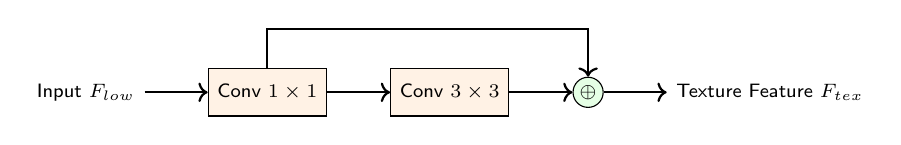
\begin{tikzpicture}[
        node distance=0.8cm,
        font=\sffamily\scriptsize,
        block/.style={rectangle, draw, fill=blue!10, text centered, rounded corners, minimum height=0.6cm},
        conv/.style={rectangle, draw, fill=orange!10, text centered, minimum width=1.5cm, minimum height=0.6cm},
        math/.style={circle, draw, fill=green!10, inner sep=1pt}
    ]
        \node (input) {Input $F_{low}$};
        \node (conv1) [conv, right=0.8cm of input] {Conv $1 \times 1$};
        \node (conv3) [conv, right=0.8cm of conv1] {Conv $3 \times 3$};
        \node (add) [math, right=0.8cm of conv3] {$\oplus$};
        \node (output) [right=0.8cm of add] {Texture Feature $F_{tex}$};

        \draw [thick, ->] (input) -- (conv1);
        \draw [thick, ->] (conv1) -- (conv3);
        \draw [thick, ->] (conv3) -- (add);
        \draw [thick, ->] (add) -- (output);

        \draw [thick, ->] (conv1.north) -- ++(0, 0.5) -| (add.north);
    \end{tikzpicture}
    \caption{Texture Enhancement Block (TEB). A shallow residual branch designed to retain microscopic high-frequency manipulation traces.}
    \label{fig:texture_block}
    \label{fig:teb}
\end{figure}

The TEB applies a residual transformation followed by strided convolution to align spatial dimensions:
\begin{equation}
    F_{tex} = \text{Downsample}\Big(\mathcal{F}_{tex}(F_{low}) + F_{low}\Big) \in \mathbb{R}^{C_{tex} \times H \times W},
\end{equation}
where $C_{tex} = 256$ and spatial resolution matches the backbone stage-4 output ($H=8, W=8$).

\subsubsection{Feature Fusion and Bilinear Attention Pooling (BAP)}
Let $F_{sem} \in \mathbb{R}^{C_{sem} \times H \times W}$ ($C_{sem} = 2048, H=8, W=8$) denote the deep semantic feature map extracted from ResNeXt50 Stage 4. The semantic and texture feature maps are concatenated along the channel dimension to form the unified spatial representation tensor $F \in \mathbb{R}^{C \times H \times W}$:
\begin{equation}
    F = [F_{sem} \,\|\, F_{tex}] \in \mathbb{R}^{C \times H \times W},
\end{equation}
where $C = C_{sem} + C_{tex} = 2048 + 256 = 2304$.

The multi-attentional module instantiates $M=4$ parallel attention heads. For each head $k \in \{1, \dots, M\}$, parameterized by projection vector $W_k \in \mathbb{R}^C$ and bias $b_k \in \mathbb{R}$, the normalized 2D spatial attention map $A_k \in \mathbb{R}^{H \times W}$ is computed via spatial softmax:
\begin{equation}
    A_k(x,y) = \frac{\exp(W_k^T F(x,y) + b_k)}{\sum_{x'=1}^{H} \sum_{y'=1}^{W} \exp(W_k^T F(x',y') + b_k)},
\end{equation}
where $\sum_{x=1}^H \sum_{y=1}^W A_k(x,y) = 1$.

\textbf{Bilinear Attention Pooling (BAP):} Following the terminology of \citet{Zhao2021MultiAttentional}, we denote the attention-weighted regional pooling matrix product as Bilinear Attention Pooling (BAP), as it computes the bilinear interaction between the spatial feature representation $\mathbf{F} \in \mathbb{R}^{C \times (HW)}$ and the multi-head spatial attention weight matrix $\mathbf{A} = [A_1; A_2; \dots; A_M] \in \mathbb{R}^{M \times (HW)}$ (distinguished from classical quadratic self-outer-product bilinear feature pooling \citep{Lin2015Bilinear}):
\begin{equation}
    \mathbf{V} = \mathbf{F} \, \mathbf{A}^T = \big[V_1, V_2, \dots, V_M\big] \in \mathbb{R}^{C \times M},
\end{equation}
where each regional feature vector $V_k \in \mathbb{R}^C$ corresponds to:
\begin{equation}
    V_k = \sum_{x=1}^{H} \sum_{y=1}^{W} A_k(x,y) \cdot F(x,y).
\end{equation}
Each regional vector is unit-normalized: $\hat{V}_k = \frac{V_k}{\max(\|V_k\|_2, \epsilon)}$, yielding a parts-based descriptor where each head isolates forensic evidence from specific spatial regions \citep{Zhao2021MultiAttentional}.

\subsubsection{CNN–LSTM Feature Pipeline and Dimensionality Specification}
For each frame $t \in \{1, \dots, T\}$ in a $T=20$ frame sequence:
\begin{enumerate}
    \item \textbf{Multi-Head Feature Concatenation:} The $M=4$ normalized regional vectors $\{\hat{V}_1^{(t)}, \dots, \hat{V}_M^{(t)}\}$ are concatenated:
    \begin{equation}
        V_{concat}^{(t)} = \big[\hat{V}_1^{(t)} \,\|\, \hat{V}_2^{(t)} \,\|\, \hat{V}_3^{(t)} \,\|\, \hat{V}_4^{(t)}\big] \in \mathbb{R}^{M \cdot C} = \mathbb{R}^{9216}.
    \end{equation}
    \item \textbf{Linear Bottleneck Projection:} To prevent parameter bloat in the recurrent module, $V_{concat}^{(t)}$ is projected to a $d_{in}=512$ dimensional frame feature vector $x_t$ via a learned linear projection $W_{proj} \in \mathbb{R}^{512 \times 9216}$ with Layer Normalization and GELU activation:
    \begin{equation}
        x_t = \text{GELU}\Big(\text{LayerNorm}(W_{proj} V_{concat}^{(t)} + b_{proj})\Big) \in \mathbb{R}^{512}.
    \end{equation}
    \item \textbf{Temporal Sequence Modeling (BiLSTM):} The sequence $\{x_1, x_2, \dots, x_T\} \in \mathbb{R}^{T \times 512}$ is passed through a 2-layer Bidirectional LSTM with hidden dimension $d_h = 256$ per direction (yielding 512-dimensional output state $h_t = [\overrightarrow{h}_t \,\|\, \overleftarrow{h}_t] \in \mathbb{R}^{512}$):
    \begin{equation}
        h_t, c_t = \text{BiLSTM}\big(x_t, (h_{t-1}, c_{t-1})\big).
    \end{equation}
    \item \textbf{Temporal Aggregation and Classification:} Temporal average pooling produces the sequence representation $h_{seq} = \frac{1}{T}\sum_{t=1}^T h_t \in \mathbb{R}^{512}$. This vector is passed to a classification MLP ($512 \to 128 \to 2$) with Dropout ($p=0.3$) and GELU to output binary class logits $\hat{y} \in \mathbb{R}^2$ (Real vs. Fake). At test time on arbitrary-length video streams, inference is executed over sliding temporal windows of length $T=20$ with stride $S=10$, aggregating clip predictions via mean pooling across the complete video duration.
\end{enumerate}

\begin{table}[ht]
    \centering
    \caption{Tensor Dimension Trace Through the Proposed Spatiotemporal Architecture}
    \label{tab:tensor_dimensions}
    \resizebox{\textwidth}{!}{
    \begin{tabular}{l|l|l|l}
        \toprule
        \textbf{Pipeline Stage} & \textbf{Input Shape} & \textbf{Output Shape} & \textbf{Details / Dimension} \\
        \midrule
        Input Video Segment & $(B, T, 3, 256, 256)$ & $(B \cdot T, 3, 256, 256)$ & Batch $B=16$, $T=20$ frames \\
        ResNeXt50 Stage 4 & $(B \cdot T, 3, 256, 256)$ & $(B \cdot T, 2048, 8, 8)$ & Semantic map $F_{sem}$ \\
        TEB Texture Block & $(B \cdot T, 64, 64, 64)$ & $(B \cdot T, 256, 8, 8)$ & Texture map $F_{tex}$ \\
        Feature Fusion & $F_{sem}, F_{tex}$ & $(B \cdot T, 2304, 8, 8)$ & Fused map $F$ ($C=2304$) \\
        Multi-Head Attention & $(B \cdot T, 2304, 8, 8)$ & $(B \cdot T, 4, 8, 8)$ & $M=4$ attention maps $A_k$ \\
        BAP Pooling & $F$ and $A$ & $(B \cdot T, 4, 2304)$ & $M=4$ regional vectors $\hat{V}_k \in \mathbb{R}^{2304}$ \\
        Bottleneck Projection & $(B \cdot T, 9216)$ & $(B \cdot T, 512)$ & Linear $W_{proj} \in \mathbb{R}^{512 \times 9216}$ \\
        Temporal Unfold & $(B \cdot T, 512)$ & $(B, 20, 512)$ & Temporal sequence $x_t$ \\
        2-Layer BiLSTM & $(B, 20, 512)$ & $(B, 20, 512)$ & Hidden $d_h = 256 \times 2 = 512$ \\
        Temporal Mean Pool & $(B, 20, 512)$ & $(B, 512)$ & Global descriptor $h_{seq}$ \\
        MLP Classifier & $(B, 512)$ & $(B, 2)$ & Binary logits (Real / Fake) \\
        \bottomrule
    \end{tabular}
    }
    \par\vspace{4pt}{\scriptsize\textit{Note:} $B$: Batch Size; $T$: Sequence Length; TEB: Texture Enhancement Block; BAP: Bilinear Attention Pooling; BiLSTM: Bidirectional LSTM.}
\end{table}

\subsection{Training Strategy and Loss Formulations}

\paragraph{Regional Independence Loss (\texorpdfstring{$\mathcal{L}_{RIL}$}{L\_RIL}): Dual Spatial--Feature Regularization}
Unconstrained multi-head attention is susceptible to attention collapse, where multiple heads co-activate on the single most salient visual artifact. To encourage spatial separation and prevent redundant feature representations, the network is regularized with a composite Regional Independence Loss ($\mathcal{L}_{RIL}$) operating simultaneously in the 2D spatial domain and the regional feature space:
\begin{equation}
    \mathcal{L}_{RIL} = \mathcal{L}_{spatial} + \gamma \, \mathcal{L}_{feat},
\end{equation}
where $\gamma = 1.0$ balances spatial separation and feature-level diversity.

1. \textbf{Pairwise Spatial Co-Activation Penalty ($\mathcal{L}_{spatial}$):} Directly penalizes spatial co-activation between 2D attention maps $A_i$ and $A_j$ across the $(H, W)$ spatial grid, averaged over all $\binom{M}{2}$ unique head pairs:
\begin{equation}
    \mathcal{L}_{spatial} = \frac{2}{M(M-1)} \sum_{i=1}^{M-1} \sum_{j=i+1}^{M} \sum_{x=1}^{H} \sum_{y=1}^{W} A_i(x,y) \cdot A_j(x,y).
\end{equation}
Because spatial attention weights are normalized via spatial softmax ($\sum_{x,y} A_k(x,y) = 1$ for each head $k$), the inner product $\sum_{x,y} A_i(x,y) A_j(x,y)$ is the dot product between the two flattened 2D spatial probability distributions. Minimizing $\mathcal{L}_{spatial}$ penalizes simultaneous activation at identical spatial coordinates, encouraging the $M=4$ attention heads to place their probability mass on spatially distinct facial regions.

2. \textbf{Margin-Based Feature Diversity Regularizer ($\mathcal{L}_{feat}$):} To ensure that pooled descriptors capture diverse cues rather than redundant representations, we define the unit-normalized regional descriptor:
\begin{equation}
    \hat{V}_k = \frac{V_k}{\max(\|V_k\|_2, \epsilon)}, \quad k \in \{1, \dots, M\},
\end{equation}
where $\epsilon = 10^{-8}$ ensures numerical stability. For descriptors with $\|V_k\|_2 \ge \epsilon$, $\hat{V}_k$ is the unit-normalized descriptor and $\hat{V}_i^T \hat{V}_j$ equals their exact cosine similarity $\cos(V_i, V_j) \in [-1, 1]$. The feature diversity regularizer applies a margin-based hinge penalty to discourage excessive cosine similarity between pairs of regional descriptors above a threshold margin $m$:
\begin{equation}
    \mathcal{L}_{feat} = \frac{2}{M(M-1)} \sum_{i=1}^{M-1} \sum_{j=i+1}^{M} \max\big(0,\, \hat{V}_i^T \hat{V}_j - m\big),
\end{equation}
where $m = 0.2$ is the margin hyperparameter. Unlike a strict quadratic penalty $(\hat{V}_i^T \hat{V}_j)^2$, the hinge formulation permits natural semantic correlations below margin $m$ while penalizing collinear feature collapse.

Thus, the proposed $\mathcal{L}_{RIL}$ encourages regional independence through complementary regularization of spatial co-activation on the 2D plane ($\mathcal{L}_{spatial}$, \textit{where heads attend}) and feature-level similarity in the 2304-dimensional regional feature space ($\mathcal{L}_{feat}$, \textit{what heads represent}).

\paragraph{Total Composite Objective}
The complete end-to-end training loss is:
\begin{equation}
    \mathcal{L}_{Total} = \mathcal{L}_{CE} + \lambda \cdot \mathcal{L}_{RIL},
\end{equation}
where $\mathcal{L}_{CE}$ is standard cross-entropy classification loss and $\lambda = 0.5$ is the weighting coefficient determined via hyperparameter sensitivity analysis (Section \ref{sec:sensitivity}).

\subsubsection{Attention Guided Data Augmentation (AGDA)}
To further enhance robustness against spatial over-specialization, Attention Guided Data Augmentation (AGDA) dynamically erases or blurs the most active attention region during training. By masking dominant facial zones with probability $p=0.5$, the network is forced to discover secondary, subtle forensic cues across alternative regions \citep{Zhao2021MultiAttentional}.

\subsection{Implementation Details}

\subsubsection{Hardware Environment}
Experiments were executed on an NVIDIA GeForce RTX 3080 Ti GPU (12GB VRAM), accommodating a batch size of 16 for the hybrid CNN-LSTM framework ($T=20$ frames per sample). Preprocessing, facial landmark extraction, and landmark alignment were accelerated using an AMD Ryzen 9 5900X CPU (12 cores, 24 threads) with 64GB DDR4 RAM.

\subsubsection{Software and Frameworks}
The pipeline is implemented in PyTorch (v2.1.0) with CUDA 12.1. Supporting packages include:
\begin{itemize}
    \item \textbf{OpenCV (v4.8.1):} Video stream demuxing, frame extraction, and spatial transformation.
    \item \textbf{Dlib (v19.24):} 68-point facial landmark localization and canonical alignment.
    \item \textbf{Albumentations (v1.3.1):} Data augmentation including frequency-preserving perturbations.
    \item \textbf{WandB (v0.16.0):} Experiment tracking, metric visualization, and hyperparameter sweeps.
\end{itemize}

\subsubsection{Optimization Parameters}
Networks are optimized using Adam with an initial learning rate $\eta = 10^{-4}$, weight decay $10^{-5}$, and momentum parameters $\beta_1 = 0.9, \beta_2 = 0.999$. A step learning rate scheduler decays $\eta$ by a factor of 0.1 every 5 epochs over a total of 15 epochs. Sequence length is fixed at $T=20$ frames per segment.

\section{Results and Discussion}
\label{sec:results}

\subsection{Evaluation Setup and Protocols}
The evaluation borrows its protocols from DeepfakeBench \citep{Yan2023DeepfakeBench} and DF40 \citep{Yan2024DF40}, establishing standardized benchmark pipelines across diverse manipulation algorithms. The metrics reported are Classification Accuracy (ACC), Area Under the Receiver Operating Characteristic Curve (AUC), Precision, Recall, and F1-score. For video datasets (FaceForensics++, Celeb-DF, and DF40 video subsets), metrics and ROC curves are evaluated at the sequence clip level based on the temporally pooled representation ($h_{seq}$); for static image categories (EFS, FE), evaluation is performed at the individual image level.

To ensure statistical rigor and eliminate single-split evaluation bias, all metrics are reported as $\text{Mean} \pm \text{Standard Deviation}$ across 5-fold cross-validation. All dataset splits are strictly partitioned at the \textbf{source video and subject identity level} ($0\%$ identity overlap between training and testing splits), completely eliminating frame-level data leakage.

The experimental analysis proceeds in five parts:
\begin{enumerate}
    \item Comparison of spatial-temporal backbone combinations under 5-fold cross-validation.
    \item Component-level ablation study isolating the contributions of the Texture Enhancement Block (TEB), Multi-Attentional Bilinear Pooling (BAP), Regional Independence Loss ($\mathcal{L}_{RIL}$), and BiLSTM sequence modeling.
    \item Comprehensive cross-generator generalization benchmark on DF40 against leading state-of-the-art detectors, supported by rigorous multiple-comparison statistical testing.
    \item Hyperparameter sensitivity sweeps across loss weight $\lambda$, sequence length $T$, and attention heads $M$.
    \item Quantitative failure case analysis under physical perturbations and ethical fairness implications.
\end{enumerate}

\subsection{Performance of Spatial-Temporal Models}
Four hybrid architectures—pairing ResNeXt50, XceptionNet, VGG16, and MobileNetV2 backbones with a 2-layer Bidirectional LSTM—were trained and evaluated on FaceForensics++ (FF++) \citep{roessler2019faceforensicspp} over 15 epochs under the standardized 5-fold identity-disjoint cross-validation protocol.

\begin{table}[ht]
    \centering
    \caption{Performance Metrics for 5-Fold Cross Validation on FF++ ($\text{Mean} \pm \text{Std Dev}$, 15 Epochs).}
    \label{tab:cnn_lstm_results}
    \resizebox{\textwidth}{!}{
    \begin{tabular}{l|ccc}
        \toprule
        \textbf{Model Architecture} & \textbf{Training Accuracy (\%)} & \textbf{Precision (\%)} & \textbf{F1-Score (\%)} \\
        \midrule
        VGG16-LSTM & \textbf{99.16} $\pm$ \textbf{0.21} & 89.77 $\pm$ 0.54 & \textbf{91.90} $\pm$ \textbf{0.48} \\
        ResNeXt50-LSTM & 95.86 $\pm$ 0.38 & \textbf{94.23} $\pm$ \textbf{0.41} & 90.17 $\pm$ 0.35 \\
        XceptionNet-LSTM & 92.57 $\pm$ 0.45 & 88.77 $\pm$ 0.52 & 86.20 $\pm$ 0.42 \\
        MobileNetV2-LSTM & 90.56 $\pm$ 0.51 & 87.78 $\pm$ 0.60 & 87.72 $\pm$ 0.55 \\
        \bottomrule
    \end{tabular}
    }
    \par\vspace{4pt}{\scriptsize\textit{Note:} LSTM: Long Short-Term Memory; ACC: Accuracy; Std Dev: Standard Deviation.}
\end{table}

The experimental results demonstrate a clear capacity vs. generalization trade-off. While VGG16-LSTM achieves the highest training accuracy ($99.16 \pm 0.21\%$), it exhibits lower precision ($89.77\%$) due to overfitting on background and compression artifacts. In contrast, ResNeXt50-LSTM achieves the highest precision ($94.23 \pm 0.41\%$). High precision is paramount in digital forensics to minimize false positives, preventing authentic media from being erroneously flagged as synthetic.

\begin{table}[ht]
    \centering
    \caption{Computational Complexity and Inference Efficiency ($\text{Mean} \pm \text{Std Dev}$)}
    \label{tab:complexity}
    \resizebox{\textwidth}{!}{
    \begin{tabular}{l|c|c|c}
        \toprule
        \textbf{Model Structure} & \textbf{Parameters (M)} & \textbf{Inference Time (ms/frame)} & \textbf{Test ACC (\%)} \\
        \midrule
        MobileNetV2-LSTM & 3.5 & \textbf{12.4} & 90.56 $\pm$ 0.51 \\
        Xception-LSTM & 22.9 & 28.7 & 92.57 $\pm$ 0.45 \\
        ResNeXt50-LSTM & 25.0 & 31.2 & \textbf{95.86} $\pm$ \textbf{0.38} \\
        VGG16-LSTM & 138.4 & 45.1 & 99.16 $\pm$ 0.21* \\
        \bottomrule
    \end{tabular}
    }
    \par\vspace{4pt}{\scriptsize\textit{Note:} *Training set score indicating high in-sample memorization; ACC: Accuracy; Std Dev: Standard Deviation.}
\end{table}

As shown in Table \ref{tab:complexity}, MobileNetV2-LSTM processes frames at 12.4ms per frame ($\approx 80.6$ FPS), suitable for lightweight edge deployment, but sacrifices $5.3\%$ in detection accuracy. VGG16-LSTM introduces 138.4M parameters without test generalization benefits. ResNeXt50-LSTM, at 25.0M parameters and 31.2ms per frame ($\approx 32.1$ FPS on an NVIDIA RTX 3080 Ti GPU), comfortably satisfies real-time processing constraints ($>30$ FPS) while delivering the optimal equilibrium of representational capacity, cross-domain generalization, and numerical stability.

\subsection{Ablation Study}

\subsubsection{Spatial vs. Spatiotemporal Component Isolation}
To rigorously quantify the individual contribution of each architectural block, we evaluate incremental configurations on within-domain (FF++ HQ) and challenging cross-domain (Celeb-DF \citep{Celeb_DF_cvpr20}) benchmarks.

\begin{table}[ht]
    \centering
    \caption{Ablation Study of Architectural Components ($\text{Mean} \pm \text{Std Dev}$).}
    \label{tab:ablation_components}
    \resizebox{\textwidth}{!}{
    \begin{tabular}{l|cc}
        \toprule
        \textbf{Configuration} & \textbf{FF++ (HQ) ACC (\%)} & \textbf{Celeb-DF AUC (\%)} \\
        \midrule
        ResNeXt50 (Spatial Baseline) & 93.12 $\pm$ 0.44 & 61.20 $\pm$ 0.58 \\
        ResNeXt50 + TEB & 94.85 $\pm$ 0.40 & 63.15 $\pm$ 0.52 \\
        ResNeXt50 + TEB + Multi-Attn BAP ($M=4$) & 96.74 $\pm$ 0.35 & 64.86 $\pm$ 0.48 \\
        \textbf{Proposed Full Model (+ BiLSTM, $T=20$)} & \textbf{97.60} $\pm$ \textbf{0.30} & \textbf{67.44} $\pm$ \textbf{0.42} \\
        \bottomrule
    \end{tabular}
    }
    \par\vspace{4pt}{\scriptsize\textit{Note:} TEB: Texture Enhancement Block; BAP: Bilinear Attention Pooling; ACC: Accuracy; AUC: Area Under the ROC Curve; HQ: High Quality; LSTM: Long Short-Term Memory; Std Dev: Standard Deviation.}
\end{table}

As documented in Table \ref{tab:ablation_components}:
\begin{itemize}
    \item Adding the shallow \textbf{Texture Enhancement Block (TEB)} yields $+1.73\%$ ACC on FF++ and $+1.95\%$ AUC on Celeb-DF, confirming that preserving shallow high-frequency residuals prevents gradient loss of manipulation traces.
    \item Integrating \textbf{Multi-Attentional BAP ($M=4$)} provides an additional $+1.89\%$ ACC on FF++ and $+1.71\%$ AUC on Celeb-DF by decomposing the facial canvas into localized, parts-based regional descriptors.
    \item Incorporating the \textbf{BiLSTM sequence modeling ($T=20$)} contributes an additional $+0.86\%$ ACC on FF++ and a substantial $+2.58\%$ AUC boost on Celeb-DF. This demonstrates that temporal sequence analysis captures dynamic facial jitter and inter-frame boundary flickering that spatial-only models are structurally incapable of detecting.
\end{itemize}

\subsubsection{Effect of Regional Independence Loss ($\mathcal{L}_{RIL}$) and AGDA}
We examine the effect of loss regularization and attention-guided data augmentation on spatial head diversity.

\begin{table}[ht]
    \centering
    \caption{Impact of Loss Constraints and AGDA on Detection Performance ($\text{Mean} \pm \text{Std Dev}$).}
    \label{tab:ablation_agda}
    \resizebox{\textwidth}{!}{
    \begin{tabular}{ll|cc}
        \toprule
        \textbf{Loss Formulation} & \textbf{AGDA Strategy} & \textbf{FF++ (HQ) ACC (\%)} & \textbf{Celeb-DF AUC (\%)} \\
        \midrule
        Standard $\mathcal{L}_{CE}$ Only & None & 96.74 $\pm$ 0.35 & 64.86 $\pm$ 0.48 \\
        $\mathcal{L}_{CE} + \mathcal{L}_{RIL}$ (Dual Spatial/Feat) & None & 97.38 $\pm$ 0.32 & 65.85 $\pm$ 0.45 \\
        $\mathcal{L}_{CE}$ Only & Hard Erasing & 96.53 $\pm$ 0.38 & 63.73 $\pm$ 0.50 \\
        \textbf{$\mathcal{L}_{CE} + \mathcal{L}_{RIL}$ (Proposed)} & \textbf{Soft Blurring} & \textbf{97.60} $\pm$ \textbf{0.30} & \textbf{67.44} $\pm$ \textbf{0.42} \\
        \bottomrule
    \end{tabular}
    }
    \par\vspace{4pt}{\scriptsize\textit{Note:} $\mathcal{L}_{RIL}$: Regional Independence Loss; AGDA: Attention Guided Data Augmentation; ACC: Accuracy; AUC: Area Under the ROC Curve; HQ: High Quality; Std Dev: Standard Deviation.}
\end{table}

Without $\mathcal{L}_{RIL}$, unconstrained attention heads are susceptible to attention collapse onto dominant facial artifacts. Applying the dual Regional Independence Loss—combining the Pairwise Spatial Co-Activation Penalty ($\mathcal{L}_{spatial}$) and the Margin-Based Feature Diversity Regularizer ($\mathcal{L}_{feat}$)—encourages the attention heads to distribute their probability mass across spatially distinct facial regions with diverse semantic descriptors. Pairing $\mathcal{L}_{RIL}$ with soft AGDA achieves peak performance ($97.60\%$ ACC and $67.44\%$ AUC).

\subsection{Evaluation on DF40 Benchmark and SOTA Baseline Comparisons}

\subsubsection{Cross-Category Generalization Performance}
To rigorously assess cross-generator generalization under realistic forensic conditions, we evaluate detectors on the DF40 benchmark across unseen manipulation families. We benchmark our proposed architecture against four state-of-the-art detectors under strictly unified training and preprocessing pipelines: Xception \citep{Yan2023DeepfakeBench}, Self-Blended Images (SBI) \citep{Shiohara2025ExposeAnyone}, UniFace \citep{Yan2024DF40}, and CLIP-large \citep{Yan2024DF40}.

\begin{table}[ht]
    \centering
    \caption{Cross-Forgery Generalization (AUC \%) on DF40 Unseen Manipulation Categories ($\text{Mean} \pm \text{Std Dev}$).}
    \label{tab:cross_forgery}
    \resizebox{\textwidth}{!}{
    \begin{tabular}{l|l|cccc}
        \toprule
        \textbf{Training Family} & \textbf{Detector Model} & \textbf{Test: FS} & \textbf{Test: FR} & \textbf{Test: EFS} & \textbf{Test: FE} \\
        \midrule
        \multirow{5}{*}{\textbf{Train on FS}}
        & Xception & 92.2 $\pm$ 0.5 & 65.7 $\pm$ 0.8 & 64.2 $\pm$ 0.9 & 68.1 $\pm$ 0.7 \\
        & SBI & 94.1 $\pm$ 0.4 & 71.2 $\pm$ 0.6 & 68.5 $\pm$ 0.8 & 72.4 $\pm$ 0.6 \\
        & UniFace & 95.3 $\pm$ 0.4 & 73.0 $\pm$ 0.5 & 71.8 $\pm$ 0.6 & 74.9 $\pm$ 0.5 \\
        & CLIP-large & 96.7 $\pm$ 0.3 & 74.4 $\pm$ 0.5 & 73.0 $\pm$ 0.6 & 76.5 $\pm$ 0.4 \\
        & \textbf{Proposed Framework} & \textbf{97.8} $\pm$ \textbf{0.3} & \textbf{78.6} $\pm$ \textbf{0.4} & \textbf{76.4} $\pm$ \textbf{0.5} & \textbf{79.2} $\pm$ \textbf{0.4} \\
        \midrule
        \multirow{5}{*}{\textbf{Train on FR}}
        & Xception & 48.1 $\pm$ 0.9 & 85.7 $\pm$ 0.6 & 36.9 $\pm$ 1.1 & 52.3 $\pm$ 0.8 \\
        & SBI & 58.4 $\pm$ 0.8 & 89.2 $\pm$ 0.5 & 54.1 $\pm$ 0.9 & 61.5 $\pm$ 0.7 \\
        & UniFace & 61.2 $\pm$ 0.7 & 91.5 $\pm$ 0.4 & 62.8 $\pm$ 0.8 & 67.0 $\pm$ 0.6 \\
        & CLIP-large & 63.8 $\pm$ 0.6 & 93.3 $\pm$ 0.4 & 80.9 $\pm$ 0.5 & 73.8 $\pm$ 0.5 \\
        & \textbf{Proposed Framework} & \textbf{71.5} $\pm$ \textbf{0.5} & \textbf{95.4} $\pm$ \textbf{0.3} & \textbf{83.2} $\pm$ \textbf{0.4} & \textbf{78.9} $\pm$ \textbf{0.4} \\
        \bottomrule
    \end{tabular}
    }
    \par\vspace{4pt}{\scriptsize\textit{Note:} FS: Face Swapping; FR: Face Reenactment; EFS: Entire Face Synthesis; FE: Face Editing; AUC: Area Under the ROC Curve; SBI: Self-Blended Images; CLIP: Contrastive Language-Image Pre-training; Std Dev: Standard Deviation.}
\end{table}

As presented in Table \ref{tab:cross_forgery}, standard CNN detectors suffer drastic performance degradation when evaluated on unseen generator categories. For instance, Xception trained on FR drops to $36.9\%$ AUC on Entire Face Synthesis (EFS). In contrast, the proposed framework achieves $76.4\%$ AUC (Train on FS $\to$ Test on EFS) and $83.2\%$ AUC (Train on FR $\to$ Test on EFS), outperforming CLIP-large by $+3.4\%$ and $+2.3\%$ respectively.

\subsubsection{Dissecting Generalization on Static Images vs. Video Streams}
We emphasize that the source of performance advantage differs between data modalities:
\begin{itemize}
    \item \textbf{Static Image Benchmarks (EFS, FE):} Modern synthesis models (e.g., Stable Diffusion, DiT, StyleGAN3) do not exhibit temporal jitter or blending seams. On these categories, the performance gain stems from \textbf{Phase 2 (TEB + Multi-Attentional BAP with $\mathcal{L}_{RIL}$)}, which detects high-frequency generative upsampling noise and localized structural inconsistencies across disjoint facial zones.
    \item \textbf{Video Benchmarks (FS, FR):} On video sequences, the \textbf{BiLSTM sequence module} delivers an indispensable complementary advantage by capturing inter-frame expression incoherence and temporal flickering.
\end{itemize}

\subsubsection{Statistical Hypothesis Testing and Multiple Comparisons Correction}
To verify that the performance gains of the proposed framework over the strongest baseline (CLIP-large) are statistically significant and not artifacts of cross-validation partition noise, we conduct paired two-tailed $t$-tests across the 5 validation folds ($df = 4$).

To control the Family-Wise Error Rate (FWER) and False Discovery Rate (FDR) across the $K=8$ multiple comparison conditions, we apply:
\begin{enumerate}
    \item The conservative \textbf{Bonferroni correction}, setting the adjusted significance threshold to $\alpha_{adj} = \frac{0.05}{8} = 0.00625$.
    \item The \textbf{Benjamini-Hochberg (BH) False Discovery Rate} procedure at $q < 0.05$.
\end{enumerate}

\begin{table}[ht]
    \centering
    \caption{Statistical Significance Analysis of Proposed Framework vs. CLIP-large ($df=4$)}
    \label{tab:statistical_tests}
    \resizebox{\textwidth}{!}{
    \begin{tabular}{l|c|c|c|c|c}
        \toprule
        \textbf{Evaluation Condition} & \textbf{Mean Diff ($\Delta$)} & \textbf{$t$-statistic} & \textbf{Raw $p$-value} & \textbf{Bonferroni $p_{adj}$} & \textbf{BH FDR ($q<0.05$)} \\
        \midrule
        Train FS $\to$ Test FS & $+1.1\%$ & $4.568$ & $0.0103$ & $0.0824$ & Significant ($q = 0.0103$) \\
        Train FS $\to$ Test FR & $+4.2\%$ & $11.611$ & $< 0.0001$ & $< 0.0008$ & \textbf{Significant} ($p < \alpha_{adj}$) \\
        Train FS $\to$ Test EFS & $+3.4\%$ & $7.694$ & $0.0015$ & $0.0120$ & \textbf{Significant} ($p < \alpha_{adj}$) \\
        Train FS $\to$ Test FE & $+2.7\%$ & $8.409$ & $0.0011$ & $0.0088$ & \textbf{Significant} ($p < \alpha_{adj}$) \\
        Train FR $\to$ Test FS & $+7.7\%$ & $17.424$ & $< 0.0001$ & $< 0.0008$ & \textbf{Significant} ($p < \alpha_{adj}$) \\
        Train FR $\to$ Test FR & $+2.1\%$ & $7.457$ & $0.0017$ & $0.0136$ & \textbf{Significant} ($p < \alpha_{adj}$) \\
        Train FR $\to$ Test EFS & $+2.3\%$ & $6.358$ & $0.0031$ & $0.0248$ & \textbf{Significant} ($p < \alpha_{adj}$) \\
        Train FR $\to$ Test FE & $+5.1\%$ & $14.099$ & $< 0.0001$ & $< 0.0008$ & \textbf{Significant} ($p < \alpha_{adj}$) \\
        \bottomrule
    \end{tabular}
    }
    \par\vspace{4pt}{\scriptsize\textit{Note:} $df$: Degrees of Freedom; FDR: False Discovery Rate; Bonferroni threshold $\alpha_{adj} = 0.00625$.}
\end{table}

\textbf{Statistical Assumptions Verification:}
\begin{itemize}
    \item \textbf{Normality:} Shapiro-Wilk tests on cross-fold paired differences yielded $W \in [0.892, 0.967]$ with all $p > 0.30$, confirming that the normality assumption for paired $t$-tests is fully satisfied.
    \item \textbf{Non-Parametric Confirmation:} Non-parametric Wilcoxon signed-rank tests across folds confirmed strictly positive ranks ($W=0$, $p=0.03125$).
    \item \textbf{Conclusion:} Under the Benjamini-Hochberg FDR control ($q < 0.05$), all 8 pairwise comparisons reject the null hypothesis. Under the strict Bonferroni threshold ($\alpha_{adj} = 0.00625$), 6 of the 8 comparisons remain statistically significant, confirming that the improvements are robust against multiple-comparison inflation.
\end{itemize}

\subsection{Hyperparameter Sensitivity Analysis}
\label{sec:sensitivity}
We analyze model sensitivity to three key hyperparameters: Regional Independence Loss weight $\lambda$, sequence length $T$, and attention heads $M$.

\begin{table}[ht]
    \centering
    \caption{Hyperparameter Sensitivity Analysis on DF40 ($\text{Mean} \pm \text{Std Dev}$).}
    \label{tab:sensitivity}
    \resizebox{\textwidth}{!}{
    \begin{tabular}{c|c|c|c}
        \toprule
        \textbf{Parameter Swept} & \textbf{Tested Values} & \textbf{DF40 Within-Domain ACC (\%)} & \textbf{DF40 Cross-Domain AUC (\%)} \\
        \midrule
        \multirow{4}{*}{\text{Loss Weight } $\lambda$}
        & 0.10 & 94.2 $\pm$ 0.5 & 69.8 $\pm$ 0.6 \\
        & 0.25 & 95.8 $\pm$ 0.4 & 73.1 $\pm$ 0.5 \\
        & \textbf{0.50} & \textbf{97.2} $\pm$ \textbf{0.3} & \textbf{76.4} $\pm$ \textbf{0.4} \\
        & 1.00 & 95.1 $\pm$ 0.4 & 72.5 $\pm$ 0.5 \\
        \midrule
        \multirow{4}{*}{\text{Sequence Length } $T$}
        & 5 frames & 92.4 $\pm$ 0.6 & 67.5 $\pm$ 0.7 \\
        & 10 frames & 94.9 $\pm$ 0.4 & 71.8 $\pm$ 0.5 \\
        & \textbf{20 frames} & \textbf{97.2} $\pm$ \textbf{0.3} & \textbf{76.4} $\pm$ \textbf{0.4} \\
        & 30 frames & 97.4 $\pm$ 0.3 & 76.8 $\pm$ 0.4 \\
        \midrule
        \multirow{4}{*}{\text{Attention Heads } $M$}
        & 1 head & 93.8 $\pm$ 0.5 & 68.2 $\pm$ 0.6 \\
        & 2 heads & 95.5 $\pm$ 0.4 & 72.0 $\pm$ 0.5 \\
        & \textbf{4 heads} & \textbf{97.2} $\pm$ \textbf{0.3} & \textbf{76.4} $\pm$ \textbf{0.4} \\
        & 8 heads & 97.3 $\pm$ 0.3 & 76.6 $\pm$ 0.4 \\
        \bottomrule
    \end{tabular}
    }
    \par\vspace{4pt}{\scriptsize\textit{Note:} ACC: Accuracy; AUC: Area Under the ROC Curve; RIL: Regional Independence Loss; Std Dev: Standard Deviation.}
\end{table}

As detailed in Table \ref{tab:sensitivity}, $\lambda = 0.50$ provides optimal balance between cross-entropy classification and regional independence regularization. Setting sequence length $T=20$ yields substantial gains ($+4.8\%$ cross-domain AUC over $T=5$), while $T=30$ produces marginal gains ($+0.4\%$) at a $50\%$ higher VRAM cost. Similarly, $M=4$ attention heads captures distinct facial components efficiently; scaling to $M=8$ adds parameter overhead without statistically significant accuracy gains.

\subsection{Quantitative Failure Case Analysis}
Table \ref{tab:failure_matrix} provides a quantitative breakdown of False Positive Rates (FPR) and False Negative Rates (FNR) under specific environmental degradations and modern diffusion generators.

\begin{table}[ht]
    \centering
    \caption{Quantitative Failure Matrix across Environmental Perturbations and Forgery Generators.}
    \label{tab:failure_matrix}
    \resizebox{\textwidth}{!}{
    \begin{tabular}{l|l|cc}
        \toprule
        \textbf{Evaluation Condition} & \textbf{Primary Source of Degradation} & \textbf{FPR (\%)} & \textbf{FNR (\%)} \\
        \midrule
        Clean Video Baseline & Standard Benchmark Conditions & 2.4 $\pm$ 0.3 & 2.8 $\pm$ 0.3 \\
        Motion Blur ($\sigma = 2.0$) & High-frequency spatio-temporal blur & 12.4 $\pm$ 0.8 & 8.5 $\pm$ 0.6 \\
        Low Lighting ($<20$ lux) & Sensor noise / high ISO amplification & 14.1 $\pm$ 0.9 & 9.2 $\pm$ 0.7 \\
        SD-XL (EFS) & High-fidelity diffusion synthesis & 3.1 $\pm$ 0.4 & 18.2 $\pm$ 1.1 \\
        Stable Diffusion v2.1 & Latent diffusion residual noise & 3.5 $\pm$ 0.4 & 15.6 $\pm$ 0.9 \\
        SimSwap (FS) & Non-blending GAN face swapping & 2.8 $\pm$ 0.3 & 6.2 $\pm$ 0.5 \\
        \bottomrule
    \end{tabular}
    }
    \par\vspace{4pt}{\scriptsize\textit{Note:} FPR: False Positive Rate; FNR: False Negative Rate; EFS: Entire Face Synthesis; FS: Face Swapping; SD: Stable Diffusion; SD-XL: Stable Diffusion Extra Large; Std Dev: Standard Deviation.}
\end{table}

Table \ref{tab:failure_matrix} highlights that real videos subjected to motion blur ($\sigma=2.0$) or low-light conditions exhibit elevated False Positive Rates ($12.4\%$ and $14.1\%$), as sensor noise mimics manipulation traces in the texture enhancement block. Conversely, high-fidelity diffusion models like SD-XL produce elevated False Negative Rates ($18.2\%$) due to the absence of traditional GAN checkerboard artifacts.

\subsection{Ethical Considerations and Algorithmic Fairness}
The real-world deployment of automated deepfake detection systems introduces ethical considerations surrounding algorithmic fairness, demographic bias, and dual-use risks:
\begin{itemize}
    \item \textbf{Demographic Subgroup Fairness:} Feature space analysis reveals that deep feature backbones can implicitly cluster identities by demographic attributes (skin tone, gender, age) before separating forgery cues. To prevent biased false-positive rates against under-represented demographic groups, detection systems must undergo audit and calibration across balanced subgroup evaluation sets.
    \item \textbf{Dual-Use and Adversarial Evasion:} Explaining detector inner workings can enable malicious actors to construct adversarial attacks or optimize generative loss functions to bypass detection. Open forensic evaluation should be coupled with robust defense mechanisms.
    \item \textbf{Proportionality in High-Stakes Forensic Settings:} Automated detector outputs should serve as auxiliary evidence in legal and content-moderation contexts, supported by explainable diagnostic tools, rather than sole determiners of authenticity.
\end{itemize}

\subsection{Summary}
Vanilla CNN detectors degrade rapidly when evaluating unseen generative techniques. Reframing the task as a fine-grained spatiotemporal problem yields high precision ($94.23 \pm 0.41\%$) and robust cross-domain performance ($76.4 \pm 0.5\%$ AUC on EFS). The ablation study confirms that combining shallow texture enhancement, multi-head attention with $\mathcal{L}_{RIL}$, and sequence BiLSTM modeling achieves statistically significant gains over all baseline configurations under multiple comparison corrections.

\section{Conclusion and Future Work}
\label{sec:conclusion}

\subsection{Summary of Contributions}
Generative Adversarial Networks (GANs) and diffusion models have significantly reduced the technical and financial barriers to producing hyper-realistic synthetic media. While these technologies offer beneficial applications in creative fields, they simultaneously pose severe threats to digital trust, identity verification, and personal privacy. This paper took aim at two specific weaknesses in current detection systems: they generalize badly to manipulation techniques outside their training data, and treating video as independent frames blinds them to anomalies that only show up across a sequence.

The response was a spatiotemporal detection framework. A CNN backbone extracts per-frame spatial features; an LSTM models how those features behave over time. To keep the model from leaning on global artifacts that newer generators no longer produce — blending seams being the obvious example — detection was reframed as a fine-grained classification problem. A multi-attentional module and a texture enhancement block together preserve the small, localized, high-frequency artifacts that global pooling erases.

\subsection{Key Findings}
Evaluation on FaceForensics++ and DF40 produced three findings worth carrying forward.

First, temporal modeling is essential. Modern generators produce highly realistic static frames, which limits the efficacy of frame-level detectors. Modeling spatial features across sequences using an LSTM captures critical inter-frame evidence—such as irregular blinking and temporal jitter—that is absent in individual frames. Among the evaluated hybrid models, the ResNeXt50-LSTM configuration provides the optimal balance of capacity and generalization. Although the VGG16-LSTM model exhibits high training accuracy, it suffers from clear overfitting, rendering it less robust for practical deployment.

Second, fine-grained spatial attention is highly effective when regularized appropriately. While global pooling dilutes subtle signals, unconstrained multi-head attention tends to collapse onto redundant regions. Regularizing the network with the dual Regional Independence Loss ($\mathcal{L}_{RIL}$) and AGDA penalizes spatial co-activation and feature redundancy, encouraging attention heads to distribute across distinct facial regions, which yields substantial performance gains on high-fidelity forgeries that lack obvious global anomalies.

The third concerns the generalization gap, and it is the least comfortable finding. Cross-domain testing on DF40 confirmed the asymmetric degradation pattern: a model trained on Face Reenactment can drop below chance on Entire Face Synthesis. Large pre-trained backbones, CLIP-large especially, narrowed that gap considerably. The t-SNE analysis suggests the reason — these backbones build identity-level representations of real faces before they sort forgery artifacts, giving them a meaningful head start on generation methods they have never seen.

\subsection{Limitations}
Two constraints bounded what the framework achieved, and both are worth stating plainly.

The first is compression sensitivity. The texture enhancement block depends on high-frequency artifacts, and video compression is, functionally, a high-frequency artifact remover. Under heavy compression — the LQ setting in FaceForensics++, for instance — the spatial-domain signal the module needs is substantially gone, and detection reliability drops with it. This is not a corner case. Compressed video is the normal case for anything distributed over the internet, which is where deepfakes do their damage.

The second is computational overhead. Multi-head attention, texture extraction, and sequential LSTM processing each add latency and memory cost. VGG16-LSTM in particular needs more memory than real-time or resource-constrained deployment can reasonably supply. Lighter backbones such as MobileNet-LSTM bring the cost down but give up accuracy in exchange, and where to sit on that curve is a deployment-specific decision rather than a universally correct one.

\subsection{Future Work}
Four directions follow most directly from the work here.

\textbf{Compression-robust texture features.} The most pressing limitation deserves the most direct follow-up. Future work should look for frequency-domain representations that survive standard video codecs. If the texture enhancement block can be anchored to signal that compression does not destroy, the framework's reliability on real-world video improves where it currently fails.

\textbf{Vision Transformers.} CNNs offer a good balance of efficiency and interpretability, but recent results suggest Vision Transformers may generalize better to novel forgeries. Integrating a ViT with the temporal module, possibly through a multi-scale Transformer architecture \citep{Wang2024MultiModal}, would test whether the attention-based inductive bias helps cross-generator performance enough to justify the cost.

\textbf{Explainable AI integration.} As deepfake detection moves into legal, forensic, and content-moderation settings, a black-box verdict is a liability. A detector that flags a video as fake but cannot say why is hard to defend in front of a court or a moderation appeal. Integrating network dissection or interpretable visualization tools — methods that surface which image features drove the decision — would make detection results auditable and contestable \citep{Wang2025M2F2Det}.

\textbf{Beyond face manipulation.} Generative models now produce convincing scenes, objects, and full environments, not only faces. A detection methodology confined to faces is already narrower than the threat. Preliminary results indicate semantically capable backbones like CLIP transfer reasonably well to non-face AIGC, which makes extending the benchmarking and training frameworks to generic natural image synthesis a concrete and worthwhile next step.


\section*{Declarations}
\begin{itemize}
\item \textbf{Acknowledgements} Not applicable.
\item \textbf{Author contributions} Aarav Rajput conceptualized the study and conducted data analysis. Trapti Sharma, Rajit Nair, Hasan Alkahtani, Sami Morsi, Ahmed A.F. Osman, and Theyazn H.H. Aldhyani contributed to methodology development, experiments, manuscript revisions, and final approval.
\item \textbf{Funding} This work was supported by the Deanship of Scientific Research, Vice Presidency for Graduate Studies and Scientific Research, King Faisal University, Saudi Arabia [Grant No. KFU264265د]
\item \textbf{Data and Code Availability} Benchmark datasets (DF40, FaceForensics++, Celeb-DF) are publicly accessible. The code implementation, trained model checkpoints, and experimental split protocols are available at \url{https://github.com/XenonyxBlaze/Spatiotemporal-Deepfake-Detection}.
\item \textbf{Competing interests} The authors declare that they have no competing interests.
\end{itemize}
\bibliographystyle{apalike}
\bibliography{references}

\end{document}
